\documentclass{article}

\usepackage{graphicx}

\title{EM Algorithm for GMM}
\author{Qi Liu}
\date{\today}

\begin{document}
	
\maketitle

\section{Data analysis}
There are 4800 samples in the training data which are divided into 2 groups. The details can be found in the figure below. It is can be observed that there are 4 Gaussian component for each group.

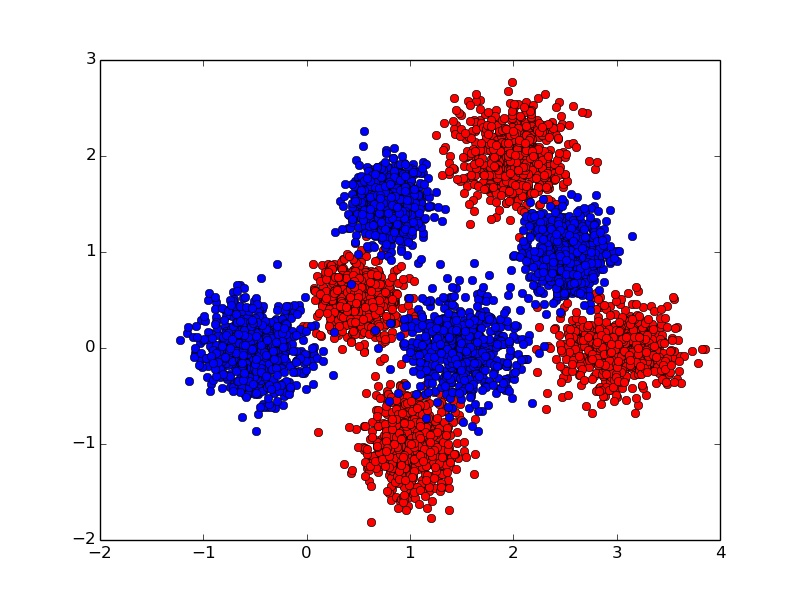
\includegraphics[width=\textwidth]{../result/train.jpg}

\section{EM training}
The GMM model for each group has been trained by 10 iterations. The initial values of $c$ are the uniform distribution. The initial value of $\mu$ are (-1, 0), (1, 0), (0, -1) and (0,1). The initial values of $\sigma$ are all the identity matrix. The log likelihood and the correct predict number of developing set have been calculated for each iteration. The left figure below correspond to the log likelihood and the right one is for correct predict number of developing set. It is can be found that EM algorithm converge very quickly due to the predict accuracy of developing set become very high at the 4th iteration.

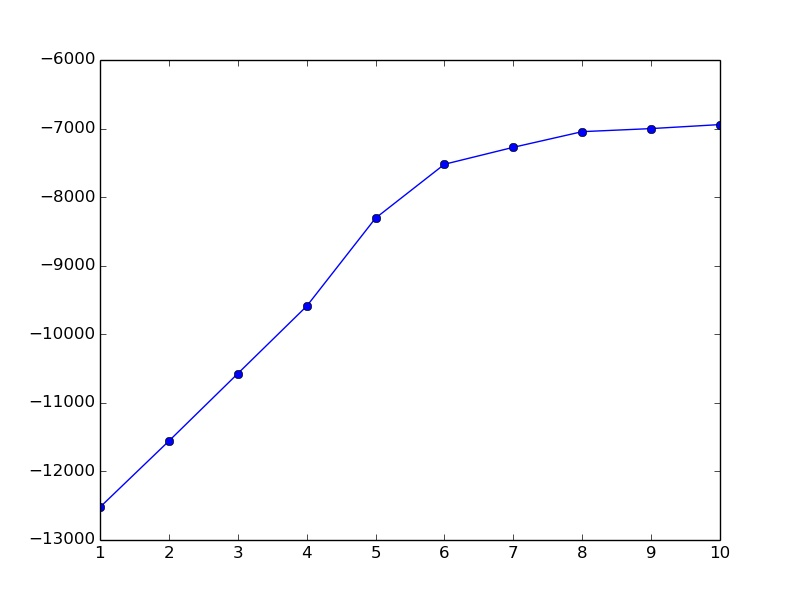
\includegraphics[width=0.5\textwidth]{../result/likelihood.jpg}
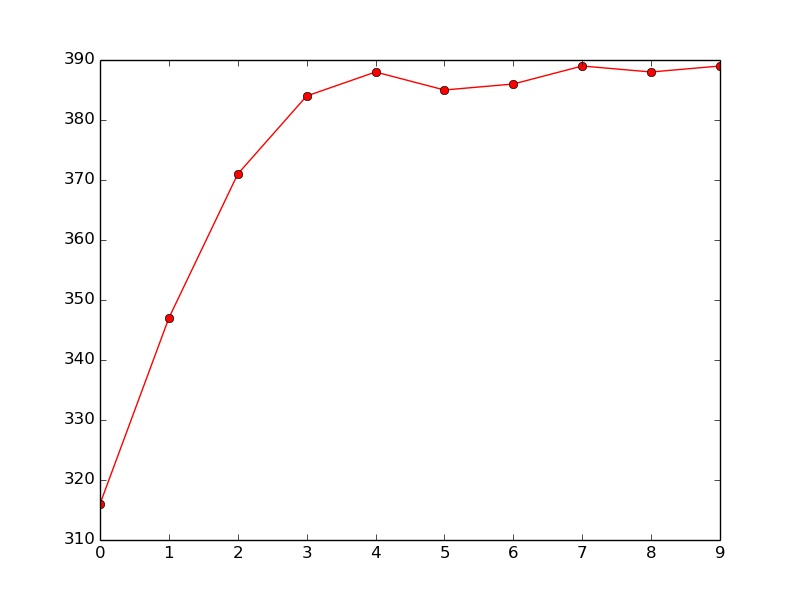
\includegraphics[width=0.5\textwidth]{../result/predict.jpg}

\section{Test set evaluation}
The evaluation result for the test set can be found in the file  \emph{result/result.txt}. The figure about grouping of test set is shown below.

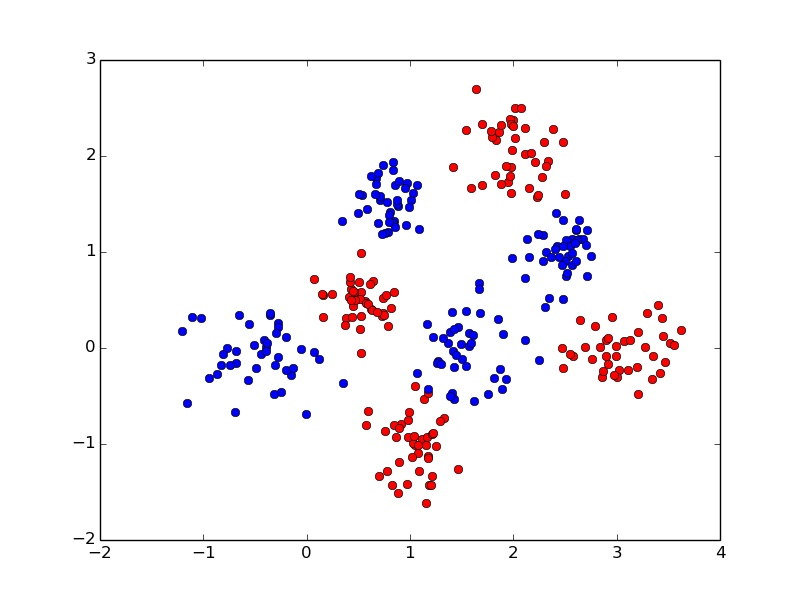
\includegraphics[width=\textwidth]{../result/test.jpg}
\end{document}